\documentclass[a4paper, twoside, 11pt]{article}
\usepackage[a4paper,top=3cm,bottom=2cm,left=3cm,right=3cm,marginparwidth=1.75cm]{geometry}

\usepackage[utf8]{inputenc}
\usepackage[T1]{fontenc}
\usepackage{textcomp}
\usepackage{amsmath, amssymb, amsthm}
%\usepackage{esint}
%\usepackage{isomath}
\usepackage{parskip}
\usepackage{stmaryrd}
\usepackage{bbold}
\usepackage{alltt}
\usepackage{graphicx}

\begingroup
    \makeatletter
    \@for\theoremstyle:=definition,remark,plain\do{%
        \expandafter\g@addto@macro\csname th@\theoremstyle\endcsname{%
            \addtolength\thm@preskip\parskip
            }%
        }
\endgroup

\theoremstyle{definition}
\newtheorem{definition}{Definition}[section]

\theoremstyle{plain}
\newtheorem{theorem}[definition]{Theorem}
\newtheorem{algorithm}[definition]{Algorithm}
\newtheorem{corollary}[definition]{Corollary}
\newtheorem{lemma}[definition]{Lemma}
\newtheorem{proposition}[definition]{Proposition}

\theoremstyle{remark}
\newtheorem*{remark}{Remark}

\newcommand{\alg}[1]{\mathsf{#1}\text{-Alg}}
\newcommand{\fun}[1]{\mathsf{#1}}
\newcommand{\cat}[1]{\mathcal{#1}}
\newcommand{\fix}[1]{\mu\fun{#1}}
\newcommand{\initial}[1]{\left<\fix{#1},ins\right>}
\newcommand{\cata}[1]{\llparenthesis #1 \rrparenthesis}
\newcommand{\ialg}[1]{\text{IAlg }\cat{#1}}
\DeclareMathOperator{\id}{\mathbb{1}}

\renewcommand{\vec}{\vectorsym}

\title{Formalising Mathematics - Project 2 \\ Category theory - Algebras over endofunctors}
\author{Omar Tahir}
\date{\today}

\begin{document}

\maketitle

In this project I formalised the notions of an algebra over an endofunctor, in particular initial objects and their properties.

\section{Algebras}

In \emph{project2.alg} I formalised the notion of the category of $\fun{F}$-algebras over some endofunctor $\fun{F} : \cat{C} \to \cat{C}$. A category is defined over the type of objects, and is a class with six fields:

\begin{itemize}
    \item The type of morphisms.
    \item The function that sends an object to its identity morphism.
    \item The function tha performs compositin of two morphisms.
    \item A proof that identity morphisms are left identities.
    \item A proof that identity morphisms are right identities.
    \item A proof that composition is associative.
\end{itemize}

An arrow $f: \left< A,a\right> \to \left< B,b\right>$ in $\alg{F}$ is an arrow in $\cat{C}$ that plays well with the algebra, i.e. it satisfies the property $f \circ a = b \circ \fun{F} f$.

Additionally I defined the forgetful functor $\fun{U} : \alg{F} \to \cat{C}$ that forgets the algebra structure.

\subsection*{Design}

I chose to implement the arrows in $\alg{F}$ as a structure with two fields, one carrying the arrow in $\cat{C}$ and another witnessing that the property above holds. Composition, identity and the thre proofs are then just the same as in the underlying category.

Unfortunately, defining arrows in this way means that arrows in $\cat{C}$ and arrows in $\alg{F}$ are distinct objects. When doing proofs on paper, this distinction is relaxed - we often write $f: \left< A,a\right> \to \left< B,b\right>$ but then say something like $f A$ which is implicitly casting down to the base category. Therefore I implemented a coercion that automatically applies $\fun{U}$ to go from an arrow in $\alg{F}$ to an arrow in $\cat{C}$.

Unfortunately, the coercion doesn't always work very well and sometimes I still have to manually use dot notation. The main reason for needing this notation is that $(\id X).h$ does not compile, even though it's correct, but $\uparrow (\id X)$ does work, and there are some situations where it's nice to have the coercion be automatic.


\section{Initial objects}

In \emph{project1.initial} I formalised some properties of initial objects in $\alg{F}$.

Going with computer science convention, I name the initial object of an $\alg{F}$ the special pair $\initial{F}$ (the algebra is usually called $in$ but that's a keyword in Lean). The catamorphism operator $\cata{-}$ takes an algebra to the unique arrow from the initial object.

I then prove several important laws:
\begin{itemize}
    \item Uniqueness: $f = \cata{a} \iff f \circ ins = a \circ F f$.
    \item Computation: $\cata{a} \circ ins = a \circ F a$.
    \item Reflection: $\id \initial = \cata{ins}$.
    \item Fusion: $k \circ \cata{a} = \cata{b}$.
\end{itemize}

These are important laws when optimising programs that use catamorphisms to execute algorithms over data structures. For example, the fusion law states that two operations can be fused into one, which means any number of traversals can be fused together into one, increasing efficiency.

In addition, I proved Lambek's lemma, which says that $\fix{F}$ is a fixed point of $\fun{F}$.

\subsection*{Problems with equality}

I encountered some very annoying issues with equality. When proving uniqueness, the reverse direction ($f = \cata{a} \iff f \circ ins = a \circ F f$) caused some trouble. The current proof is

\begin{figure}[htpb]
    
\includegraphics[width=0.5\textwidth]{pic1.png}
\end{figure}

which uses the fact that any two arrows from an initial object are equal. But the original proof was

\begin{figure}[htpb]
    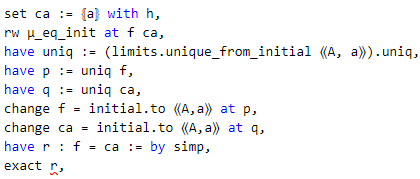
\includegraphics[width=0.6\textwidth]{pic2.png}
\end{figure}

with a final tactic state of

\newpage

\begin{figure}[htpb]
    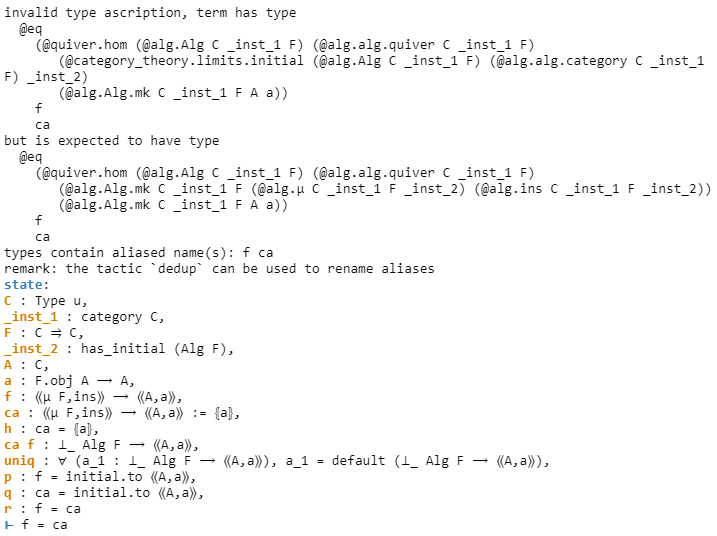
\includegraphics[width=0.85\textwidth]{pic3.png}
\end{figure}

Note the aliased \texttt{f} and \texttt{ca} - the theorem $\mu$\texttt{\_eq\_init} changed the type of the equality, which meant that while I have a valid term of type \texttt{f=ca} the actual type of that equality is not correct. This is a problem I have also struggled with in Idris, a language like Haskell but with theorem proving capabilities.


\section{Intial objects again}

In \emph{project1.initial2} I defined the $\mu$ fixpoint operator in a different way.

$\mu$ is actually a higher-order functor of the for $\cat{C}^{\cat{C}} \to \cat{C}$. In the previous section I defined $\mu$ as a function, but here I decided to make it an actual functor.

\subsection{Design}

The functor only operates on functors whose algebra category has an initial object. This is something hand-waved away when we do this on paper - we just say ``$\mu$ takes functors $\fun{F}$ to their initual objects in $\alg{F}$ provided they have one''. As far as Lean is concerned, there are two crimes here. Firstly, $\mu$ is most certainly not $\cat{C}^{\cat{C}} \to \cat{C}$, because there are functors whose category of algebras does not have an initial object. Secondly, the initial object in $\alg{F}$ is $\initial{F}$, not just $\fix{F}$. We move between these trivially but Lean requires this to be spelt out explicitly.

Therefore I defined a new category $\ialg{C}$ that is the category of endofunctors over $\cat{C}$ whose categories of algebras have initial objects. The objects are pairs whose first element is the functor $\fun{F}$ and whose second element is an instance of the \texttt{has\_initial} typeclass for $\alg{F}$. The morphisms are natural transformations on $\cat{C}$.

Using this, the desired functor is $\text{Mu} : \ialg{C} \to \cat{C}$, that sends $\fun{F}$ to $\fix{F}$ and sends natural transformations $\alpha : \fun{F} \to \fun{G}$ to $\cata{ins \circ \alpha(\fix{G})}$.

Unfortunately I was unable to prove the base functor fusion law, which says that $\cata{a} \circ \text{Mu } \alpha = \cata{a \circ \alpha A}$.


\end{document}